\documentclass[11pt]{article}
\usepackage{amsmath, amsthm, amsfonts,amssymb}
\usepackage[utf8]{inputenc}
\usepackage[spanish]{babel}
\usepackage{multicol}
\usepackage{listings}
\lstset{basicstyle=\footnotesize\ttfamily,breaklines=true}
\usepackage{alltt}
\usepackage{graphicx}
\usepackage{subfigure}
\usepackage{subfig}
\usepackage{float}
\usepackage{url}
\usepackage{enumerate}
\usepackage{framed}
\usepackage{color}
\usepackage{wrapfig}\definecolor{shadecolor}{RGB}{250,250,250}
\usepackage{framed}
\usepackage{epstopdf}
\setlength\parindent{0pt}
\usepackage{listings}
\usepackage{color} %red, green, blue, yellow, cyan, magenta, black, white
% Operadores matemáticos y simbolos
\DeclareMathOperator{\dive}{div}
\DeclareMathOperator{\trace}{trace}
\DeclareMathOperator{\tr}{tr}
\DeclareMathOperator{\symm}{symm}
\DeclareMathOperator{\sk}{skew}
\DeclareMathOperator{\grad}{grad}
\DeclareMathOperator{\Grad}{Grad}
\DeclareMathOperator{\curl}{curl}
\DeclareMathOperator{\Curl}{Curl}
\def\R{\mbox{\(\mathbb{R}\)}}
\def\E{\mbox{\(\mathbb{E}\)}}
\def\P{\mbox{\(\mathbb{P}\)}}
\def\I{\mbox{\(\mathbb{I}\)}}
\def\L{\mbox{\(\mathbb{L}\)}}
\def\dx{\mbox{\(\,\mathrm{d}x\)}}
\usepackage{geometry}
\geometry{left=2.5cm, right=2.5cm, top=2cm, bottom=3cm}
\begin{document}
\begin{figure}
\begin{minipage}{2.5cm}

\includegraphics[width=0.8\textwidth]{./figures/LogoUC-BN}
\end{minipage}
\begin{minipage}{14.5cm}
\vspace{4mm}
{\sc PONTIFICIA UNIVERSIDAD CAT\'OLICA DE CHILE}\\
{\sc FACULTAD DE INGENIER\'IA} \\
IEE - 2714 \ Fundamentos de Procesamiento de Imágenes \\
Profesor: Cristián Tejos (ctejos@ing.puc.cl) \\
Nombre Alumno: Alberto Valdés (anvaldes@uc.cl). \\

\vspace{-8mm}
\hrulefill
\end{minipage}
\end{figure}
\phantom{""}
\vspace{-10mm}
\normalsize

\begin{center}
	\huge{Tarea 1}\\
	\normalsize Parte 2 
\end{center}

\providecommand{\abs}[1]{\lvert#1\rvert}

\providecommand{\norm}[1]{\lVert#1\rVert}

\section{Explicación de lo realizado}

Primero que todo, es importante notar que utilizaremos $256$ puntos de control ($L = 256 $). \\

Realizamos esta analísis sobre 2 imagenes. Una imagen es personal y la otra es de un futbolista. Para cada imagen, en primer lugar la mostramos en RGB y en escala de grises. Después de eso, lo que realizamos fue una ecualización de la imagen en escala de grises y luego para el caso RGB realizamos una ecualización para cada canal y luego unimos tales ecualizaciones en una sola imagen. Esta ecualización se realizo utilizando el resultado de que: \\

Sea  $F(x)$ la función de distribución acumulada de una variable aleatoria X, entonces: 

\[ (L-1) \cdot F(X) \sim Uniforme[0,L-1] \]

Una vez hecha la ecualización, lo que realizamos fue la especificación para 2 casos, y esto lo hicimos utilizando que sea $ G $ la función de distribución acumulada de una variable aleatoria $ Y $, entonces si consideramos una variable aleatoria $ U \sim Uniforme[0,1] $, entonces:

\[ G^{-1}(U) \text{ distribuye como } Y \]

Y como en el paso anterior llegamos a que ahora los pixeles distruyen $Uniforme[0,L-1]$, entonces para la especificación lo que hacemos es dividir cada pixel en $255$ y luego le aplicamos $ G^{-1} $ y así obtenemos finalmente que los pixeles distribuyen como $ Y $. \\

\textbf{i. Exponencial:} Nosotros sabemos que la distribución de probabilidad acumulada es:

\[ F(x) = 1 - e^{-\lambda x} \ \Rightarrow \ F^{-1}(u) = - \frac{1}{\lambda} \cdot ln (1-u) \]

Notemos que $ \frac{1}{\lambda} = media $, entonces:

\[ F^{-1}(u) = - media \cdot ln(1-u) \]

Y nosotros para nuestra especificación utilizamos que la media fuera $ 100 $, entonces la función a utilizar es:

\[ F^{-1}(u) = - 100 \cdot ln(1-u) \]

\newpage

\textbf{ii. Triangular:} La distribución triangular que utilizamos fue una que vale $ 0 $ desde $0$ hasta $ x = l $. Desde $ x = l $ hasta $ x = 2l $ crece hasta llegar a $ \frac{1}{l} $ y luego desde $ x = 2l $ hasta $ 3l $ descrece hasta llegar a $0$ nuevamente, y finalmente para todo valor mayor a $ 3l $ la distribución vale $0$. \\

Para esta distribución, tenemos que la inversa de la distribución acumulada es:

\begin{center}

$   F^{-1}(u) = 
   \begin{cases} 
      l \cdot [1 + \sqrt{2u}]              & \mbox{si } u \in \left[0, \frac{1}{2} \right]   \\
      l \cdot [3 - \sqrt{2-2u}] & \mbox{si } u \in \left[ \frac{1}{2}, 1 \right]
   \end{cases} $

\end{center}

Y lo que nosotros utilizamos fue que $ l = 85 $. \\

\section{Resultados}

\textbf{a) Imagen personal:} \\

\textbf{i) Imagenes:}

\begin{center}
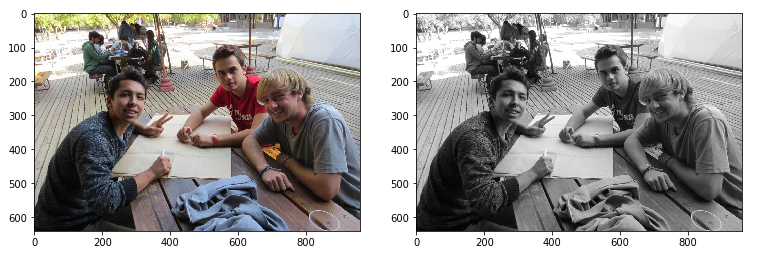
\includegraphics[width=0.8\textwidth]{./figures/beto_normal}
\end{center}

\textbf{Comentarios:} Aquí lo que mostramos fue nuestra imagen personal en RGB y en escala de grises. \\

$ \ $ 

\begin{center}
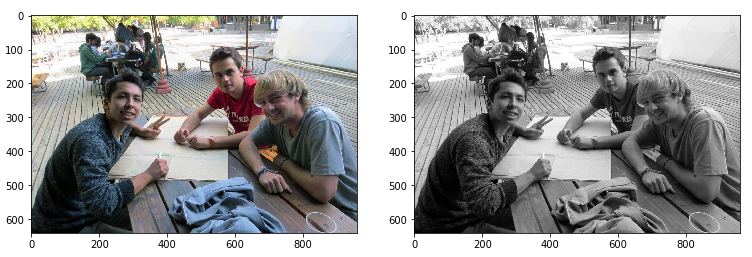
\includegraphics[width=0.8\textwidth]{./figures/beto_ecualizado}
\end{center}

\textbf{Comentarios:} Aquí estamos mostrando la imagen personal ecualizada tanto para el caso RGB como para el caso en escala de grises. \\

$ \ $ 

\begin{center}
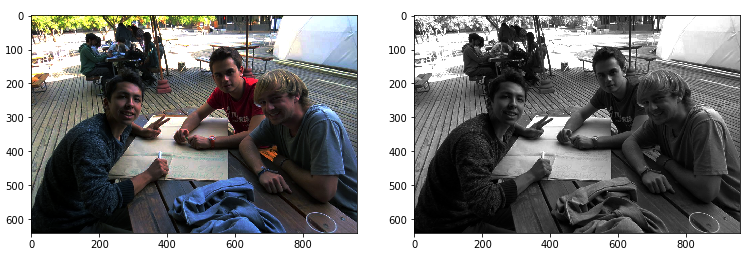
\includegraphics[width=0.8\textwidth]{./figures/beto_exponencial}
\end{center}

\textbf{Comentarios:} Aquí estamos mostrando ambas imagenes con la especificación exponencial. \\

$ \ $ 

\begin{center}
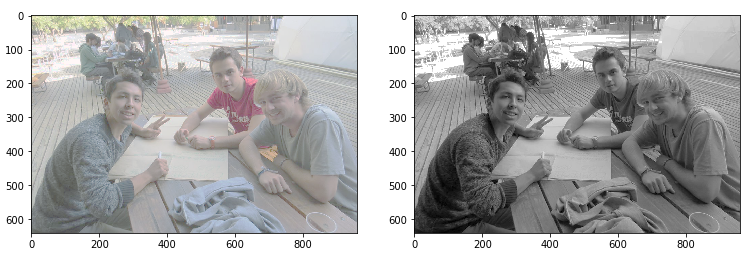
\includegraphics[width=0.8\textwidth]{./figures/beto_triangular}
\end{center}

\textbf{Comentarios:} Aquí estamos mostrando ambas imagenes con la especificación triangular. \\


$ \ $ 

\textbf{ii) Histogramas y distribuciones acumuladas:} \\

Para cada caso tenemos que en la parte izquierda esta el histograma y en la parte derecha esta la distribución acumulada. Estos histogramas y distribuciones acumuladas corresponden a la imagen en escala de grises. \\


\begin{center}
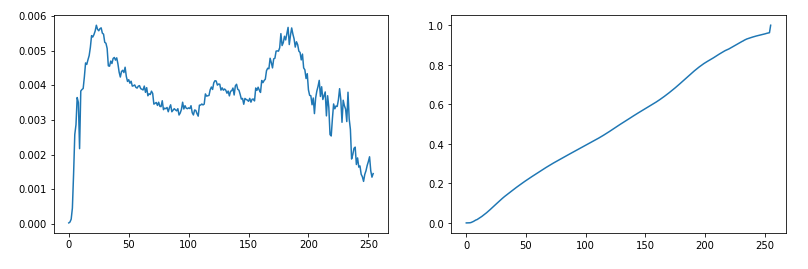
\includegraphics[width=0.8\textwidth]{./figures/grafico_beto_normal}
\end{center}

\textbf{Comentarios:} Acá presentamos el histograma y distribución acumulada para la imagen normal en escala de grises. \\

\begin{center}
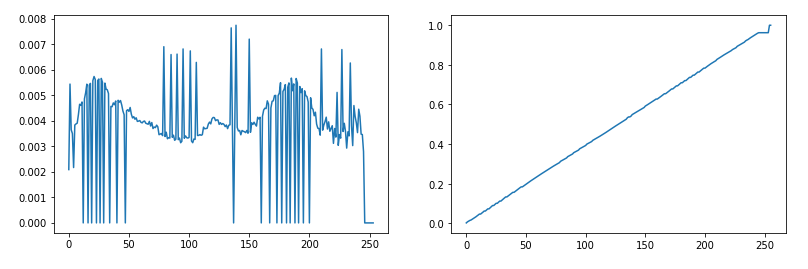
\includegraphics[width=0.8\textwidth]{./figures/grafico_beto_ecualizado}
\end{center}

\textbf{Comentarios:} Acá presentamos el histograma y distribución acumulada para la imagen ecualizada en escala de grises. En el grafico de distribución acumulada se puede observar claramente que los pixeles distribuyen de manera uniforme, pues la distribución acumulada es una recta. \\

\begin{center}
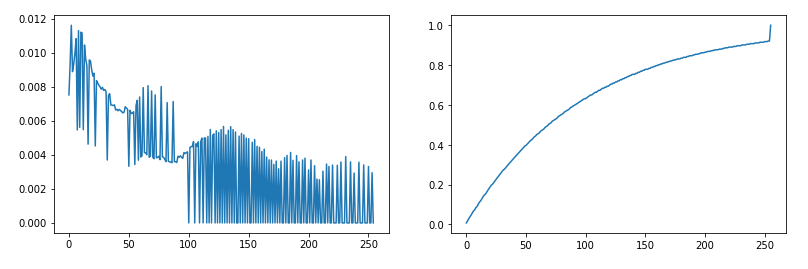
\includegraphics[width=0.8\textwidth]{./figures/grafico_beto_exponencial}
\end{center}

\textbf{Comentarios:} Acá presentamos el histograma y distribución acumulada para la imagen especificada   en escala de grises según la distribución exponencial. En el grafico de distribución acumulada se puede observar claramente que los pixeles distribuyen de manera exponencial, pues la distribución acumulada es igual al de una distribución exponencial. \\

\begin{center}
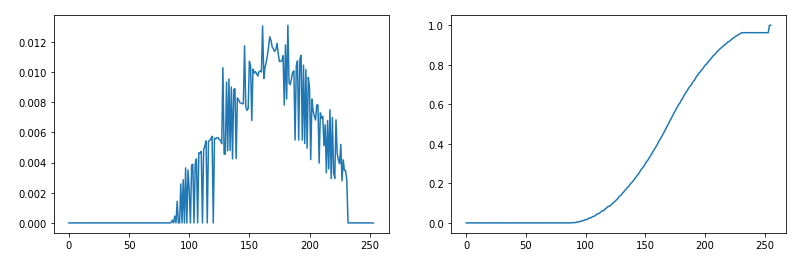
\includegraphics[width=0.8\textwidth]{./figures/grafico_beto_triangular}
\end{center}

\textbf{Comentarios:} Acá presentamos el histograma y distribución acumulada para la imagen especificada   en escala de grises según la distribución triangular. En el grafico de histograma se puede observar claramente que los pixeles distribuyen de manera triangular, pues desde $ x = 0 $ hasta $ x = 85 $ el histograma vale $ 0 $, desde $ x = 85 $ a $ x = 170 $ la distribución crece desde $ 0 $ hasta $ \frac{1}{85} $, y desde $ x = 170 $ hasta $ x = 255 $ la distribución decrece desde $ \frac{1}{85} $ hasta $ 0 $. Por otra parte, también la distribución de probabilidad acumulada es igual al de una distribución triangular. \\

\newpage

\textbf{b) Imagen de futbolista:} \\

\textbf{i) Imagenes:} \\


\begin{center}
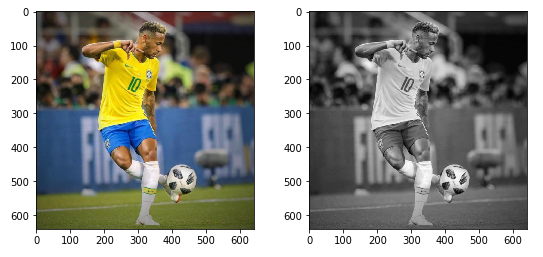
\includegraphics[width=0.6\textwidth]{./figures/neymar_normal}
\end{center}

\textbf{Comentarios:} Aquí lo que mostramos fue la imagen en RGB y en escala de grises. \\

\begin{center}
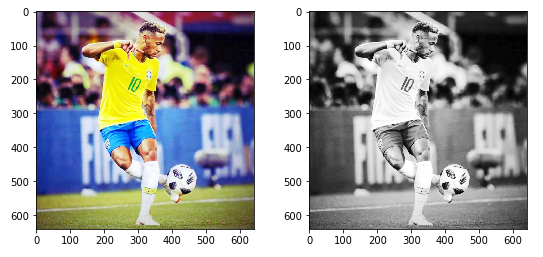
\includegraphics[width=0.6\textwidth]{./figures/neymar_ecualizado}
\end{center}

\textbf{Comentarios:} Aquí estamos mostrando la imagen ecualizada tanto para el caso RGB como para el caso en escala de grises. \\

\begin{center}
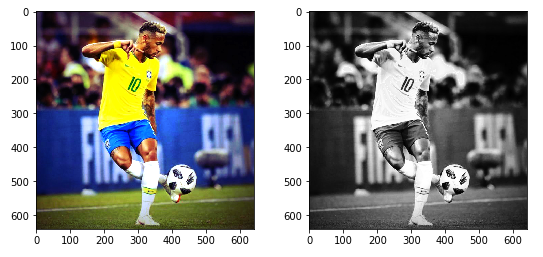
\includegraphics[width=0.6\textwidth]{./figures/neymar_exponencial}
\end{center}

\textbf{Comentarios:} Aquí estamos mostrando ambas imagenes con la especificación exponencial. \\

\begin{center}
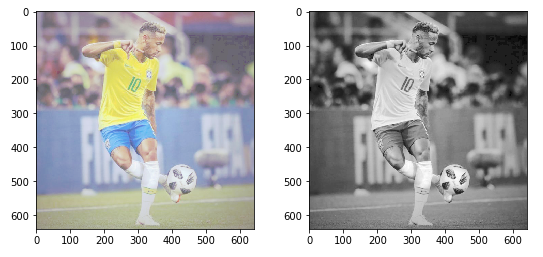
\includegraphics[width=0.6\textwidth]{./figures/neymar_triangular}
\end{center}

\textbf{Comentarios:} Aquí estamos mostrando ambas imagenes con la especificación triangular. \\


\textbf{ii) Histogramas y distribuciones acumuladas:} \\

Para cada caso tenemos que en la parte izquierda esta el histograma y en la parte derecha esta la distribución acumulada. Estos histogramas y distribuciones acumuladas corresponden a la imagen en escala de grises. \\

\begin{center}
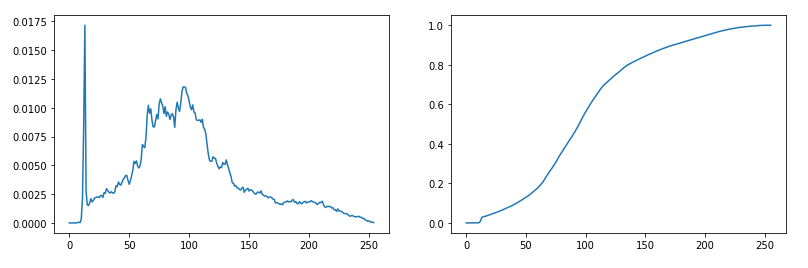
\includegraphics[width=0.8\textwidth]{./figures/grafico_neymar_normal}
\end{center}

\textbf{Comentarios:} Acá presentamos el histograma y distribución acumulada para la imagen normal en escala de grises. \\


\begin{center}
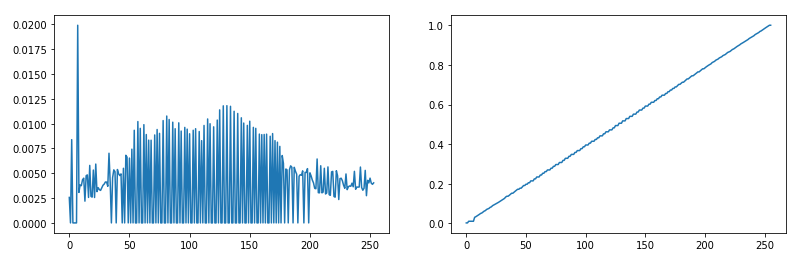
\includegraphics[width=0.8\textwidth]{./figures/grafico_neymar_ecualizado}
\end{center}

\textbf{Comentarios:} Acá presentamos el histograma y distribución acumulada para la imagen ecualizada en escala de grises. En el grafico de distribución acumulada se puede observar claramente que los pixeles distribuyen de manera uniforme, pues la distribución acumulada es una recta. \\

\begin{center}
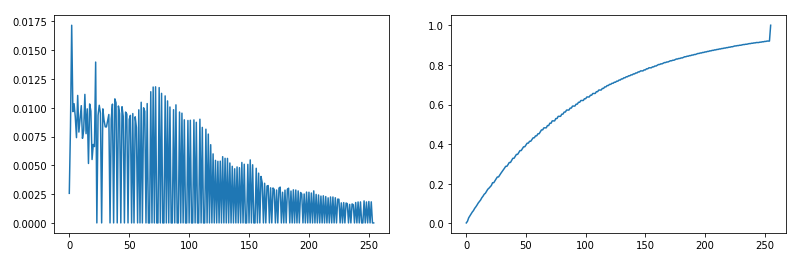
\includegraphics[width=0.8\textwidth]{./figures/grafico_neymar_exponencial}
\end{center}

\textbf{Comentarios:} Acá presentamos el histograma y distribución acumulada para la imagen especificada   en escala de grises según la distribución exponencial. En el grafico de distribución acumulada se puede observar claramente que los pixeles distribuyen de manera exponencial, pues la distribución acumulada es igual al de una distribución exponencial. \\

\begin{center}
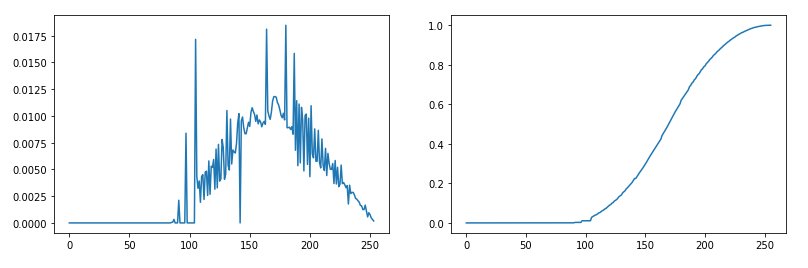
\includegraphics[width=0.8\textwidth]{./figures/grafico_neymar_triangular}
\end{center}

\textbf{Comentarios:} Acá presentamos el histograma y distribución acumulada para la imagen especificada   en escala de grises según la distribución triangular. En el grafico de histograma se puede observar claramente que los pixeles distribuyen de manera triangular, pues desde $ x = 0 $ hasta $ x = 85 $ el histograma vale $ 0 $, desde $ x = 85 $ a $ x = 170 $ la distribución crece desde $ 0 $ hasta $ \frac{1}{85} $, y desde $ x = 170 $ hasta $ x = 255 $ la distribución decrece desde $ \frac{1}{85} $ hasta $ 0 $. Por otra parte, también la distribución de probabilidad acumulada es igual al de una distribución triangular. \\




\end{document}
